\section{Resultados}
\label{resultados}

\subsection{Estrutura do grafo e avaliação específica do Leiden}

\begin{table*}[!t]
\centering
\caption{Estrutura dos grafos ($k = 40$, 3.630 vértices) e avaliação específica do Leiden, por janela e distância: arestas $|E|$, grau médio $\bar{k}$, fração no maior componente (MC), coeficiente de agrupamento $C$ e caminho médio $\ell$ no maior componente, modularidade $Q$, comunidades com $\geq 30$ alunos e faixa de evasão entre elas, V de Cramér comunidade $\times$ desfecho, maior V entre 1.000 permutações do desfecho (nulo; $p = 0{,}001$ em todas), fração de arestas entre alunos com o mesmo desfecho (52\% ao acaso) e assortatividade pelo desfecho $r_y$.}
\label{tab-grafo}
\small
\setlength{\tabcolsep}{4.2pt}
\begin{tabular}{@{}llrrrrrrcccccc@{}}
\toprule
\textbf{Janela} & \textbf{Distância} & $|E|$ & $\bar{k}$ & MC & $C$ & $\ell$ & $Q$ & \textbf{Com.} & \textbf{Evasão} & $V$ & $V$ \textbf{nulo} & \textbf{Mesmo desf.} & $r_y$ \\
\midrule
Matrícula    & Gower      & 39.980 & 22,0 & 99,9\% & 0,30 & 4,1 & 0,67 & 12 & 19--70\% & 0,32 & 0,10 & 61\% & 0,16 \\
             & Associação & 41.742 & 23,0 & 96,2\% & 0,41 & 5,3 & 0,84 & 16 & 19--67\% & 0,33 & 0,10 & 61\% & 0,17 \\
Fim do 1º sem. & Gower    & 37.318 & 20,6 & 99,7\% & 0,27 & 4,1 & 0,64 & 11 & 13--83\% & 0,46 & 0,09 & 73\% & 0,41 \\
             & Associação & 36.564 & 20,1 & 95,7\% & 0,39 & 5,3 & 0,82 & 18 & 4--96\%  & 0,58 & 0,12 & 78\% & 0,52 \\
Fim do 2º sem. & Gower    & 37.469 & 20,6 & 99,8\% & 0,27 & 4,1 & 0,65 & 13 & 8--92\%  & 0,61 & 0,10 & 79\% & 0,53 \\
             & Associação & 31.734 & 17,5 & 95,1\% & 0,39 & 5,6 & 0,80 & 16 & 5--100\% & 0,62 & 0,10 & 83\% & 0,62 \\
\bottomrule
\end{tabular}
\end{table*}

\begin{figure*}[!t]
\centering
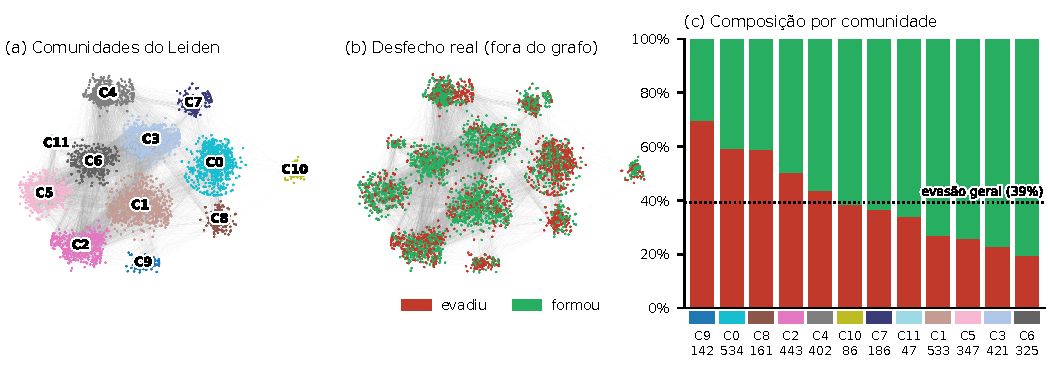
\includegraphics[width=\textwidth]{figuras/15_grafo_1_matricula_gower.pdf}
\caption{Grafo kNN mútuo ($k = 40$) da matrícula com a distância de Gower: (a) comunidades do Leiden; (b) os mesmos alunos coloridos pelo desfecho real, que não entrou na construção do grafo; (c) composição de cada comunidade, com a marca de cor da comunidade em (a). Vermelho é sempre evasão e verde, formatura.}
\label{fig-grafo}
\end{figure*}

Os seis grafos são esparsos (densidade de 0,48\% a 0,63\%). Com Gower, ficam praticamente conexos; com a distância por associação, de 4\% a 5\% dos alunos, com combinações raras de categorias, formam componentes próprios, porque essa distância pesa mais as categorias raras (Tabela~\ref{tab-grafo}). O agrupamento é de 50 a 80 vezes o de um grafo aleatório de mesma densidade, e o caminho médio é curto: são vizinhanças coesas, o que favorece a detecção de comunidades.

Na avaliação específica, as comunidades separam a evasão muito acima do acaso nas seis combinações: o V observado é de três a seis vezes o maior V obtido com o desfecho embaralhado. A separação cresce ao longo da trajetória (V de 0,32--0,33 na matrícula, 0,46--0,58 no 1º semestre e 0,61--0,62 no 2º), assim como a homofilia (de 61\% para 83\% das arestas entre alunos com o mesmo desfecho, contra 52\% ao acaso). A distância por associação gera comunidades mais coesas ($Q$ maior) em todas as janelas e mais separadas no 1º semestre. A Figura~\ref{fig-grafo} mostra a matrícula: as regiões de cor de (b) coincidem com as comunidades de (a), mesmo sem o desfecho ter entrado no grafo, e a evasão vai de 19\% (C6) a 70\% (C9).

\subsection{Avaliação comum: as quatro variações na mesma régua}

\begin{table*}[!t]
\centering
\caption{Avaliação comum: média nas mesmas 50 divisões 80/20 de F1 macro, AUC e revocação da evasão (Rev.), por janela; desvios-padrão de 0,009 a 0,018 (F1 e AUC). Classificador trivial: F1 = 0,38 e AUC = 0,50.}
\label{tab-comparacao}
\small
\setlength{\tabcolsep}{5pt}
\begin{tabular}{@{}lccccccccc@{}}
\toprule
 & \multicolumn{3}{c}{\textbf{Matrícula}} & \multicolumn{3}{c}{\textbf{Fim do 1º semestre}} & \multicolumn{3}{c}{\textbf{Fim do 2º semestre}} \\
\cmidrule(lr){2-4}\cmidrule(lr){5-7}\cmidrule(lr){8-10}
\textbf{Abordagem} & F1 & AUC & Rev. & F1 & AUC & Rev. & F1 & AUC & Rev. \\
\midrule
\textcolor{corLeiden}{\textbf{V1}} Gower + Leiden          & 0,631 & 0,679 & 0,65 & 0,701 & 0,763 & 0,68 & 0,762 & 0,833 & 0,66 \\
\textcolor{corLeiden}{\textbf{V3}} Associação + Leiden     & 0,634 & 0,687 & 0,68 & 0,740 & 0,827 & 0,73 & 0,760 & 0,849 & 0,73 \\
\textcolor{corSage}{\textbf{V2}} Gower + GraphSAGE         & 0,675 & 0,730 & 0,62 & 0,863 & 0,925 & 0,81 & 0,894 & 0,946 & 0,85 \\
\textcolor{corSage}{\textbf{V4}} Associação + GraphSAGE    & 0,674 & 0,733 & 0,64 & 0,865 & 0,923 & 0,81 & 0,893 & 0,946 & 0,85 \\
\bottomrule
\end{tabular}
\end{table*}

\begin{figure}[!ht]
\centering
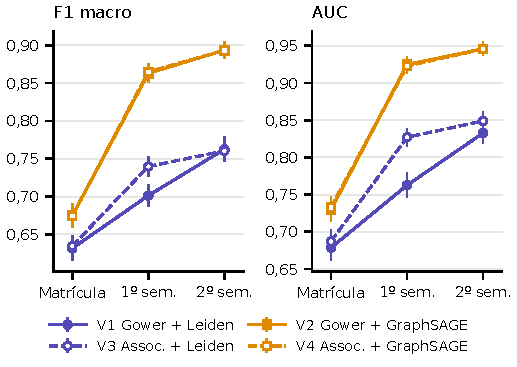
\includegraphics[width=\columnwidth]{figuras/14_comparacao_8020.pdf}
\caption{F1 macro e AUC (média $\pm$ desvio-padrão em 50 divisões 80/20) ao longo das três janelas. Roxo: Leiden; âmbar: GraphSAGE; linha cheia: Gower; tracejada: associação. As duas GraphSAGE ficam sobrepostas.}
\label{fig-comparacao}
\end{figure}

A Tabela~\ref{tab-comparacao} e a Figura~\ref{fig-comparacao} mostram as quatro variações na mesma régua. Todas ficam muito acima do classificador trivial, e o teste de Friedman rejeita a igualdade das quatro variações nas três janelas ($p < 0{,}001$). Quatro padrões se repetem.

\textbf{(i) O método pesa mais que a distância.} Com a mesma distância, a GraphSAGE supera o Leiden em 98\% a 100\% das divisões, em todas as janelas: por 0,04 de F1 na matrícula e por 0,13 a 0,16 depois. O Leiden resume cada aluno em uma de 11 a 18 comunidades, ganhando interpretabilidade e perdendo resolução individual.

\textbf{(ii) A distância só importa para o Leiden.} Com a associação, o Leiden ganha AUC em todas as janelas: 0,01 na matrícula (66\% das divisões), 0,06 no 1º semestre (100\%) e 0,02 no 2º (90\%); no F1, o ganho só aparece no 1º semestre (0,04). Entre as duas GraphSAGE, a diferença não passa de 0,003.

\textbf{(iii) Na matrícula, o Leiden encontra mais evadidos.} Com menos informação, a atribuição pela comunidade tem revocação maior que a GraphSAGE (0,65--0,68 contra 0,62--0,64), embora com F1 menor: o limiar pela taxa da comunidade marca como risco grupos inteiros. A partir do 1º semestre, a GraphSAGE encontra de 81\% a 85\% dos evadidos, contra 66\% a 73\% do Leiden. Na avaliação específica, a GraphSAGE é estável: desvio-padrão de 0,010 a 0,016 em F1 entre as divisões, diferença de no máximo 0,003 entre as duas distâncias e de no máximo 0,008 com $k = 20$ e $k = 60$.

\textbf{(iv) O 1º semestre concentra o ganho.} Da matrícula para o 1º semestre, o F1 da GraphSAGE sobe 0,19; do 1º para o 2º, só 0,03. Esperar o 2º semestre acrescenta pouco acerto e consome metade do tempo de intervenção.

\subsection{Perfis identificados}

\textbf{Matrícula.} As duas distâncias apontam o mesmo grupo de maior risco. Com Gower (C9 na Figura~\ref{fig-grafo}), são 142 alunos com 70\% de evasão: 83\% têm mãe ou pai com escolaridade desconhecida e 61\% têm 25 anos ou mais. Com associação, o grupo tem 166 alunos e 67\% de evasão, e 95\% dos alunos de C9 estão nele, embora as partições concordem só em parte no geral (ARI de 0,33). A escolaridade desconhecida atinge só 4\% dos alunos; a comunidade revela esse grupo sem que se indique qual variável olhar. Seguem 534 alunos mais velhos que ingressaram pelo concurso para maiores de 23 anos (C0, 59\%) e 161 que já têm curso superior (C8, 59\%). \textbf{Fim do 1º semestre.} Surgem grupos extremos: com Gower, 395 alunos com notas e aprovações cerca de 1 desvio-padrão abaixo da média, 65\% deles com mensalidade atrasada, têm 83\% de evasão; com associação, 267 alunos com notas 1,5 desvio-padrão abaixo da média chegam a 96\%. \textbf{Sucesso.} Na matrícula, as comunidades de menor evasão (19\% a 26\%) reúnem alunos mais jovens, quase todos deslocados e, em geral, mulheres que ingressaram pela 1ª fase do contingente geral. No 1º semestre, a associação isola três comunidades com 4\% a 8\% de evasão: mulheres jovens com notas acima da média, todas bolsistas em duas delas.

\subsection{Robustez}
\label{ssec:robustez}

Com $k = 20$ e $k = 60$ (10 divisões 80/20 cada, na matrícula e no 1º semestre), o F1 e a AUC de cada variação mudam no máximo 0,022; a GraphSAGE continua acima do Leiden, e a associação continua à frente no Leiden. Entre as distâncias, as partições concordam só em parte (ARI de 0,33, 0,21 e 0,26 nas três janelas), mas o grupo de maior risco da matrícula é o mesmo. Os achados não dependem do $k$ nem da distância.

\subsection{Perfis semelhantes, destinos diferentes}

Na matrícula, 39\% das arestas (15.560 pares com Gower e 16.268 com associação) ligam alunos parecidos que tiveram desfechos opostos. A Figura~\ref{fig-gemeos} compara, em cada par, o aluno que evadiu com o que se formou. Nos controles (idade e nota de admissão), os dois quase não diferem. No 1º semestre, o que evadiu teve 2,7 aprovações contra 6,2, nota média 7,7 contra 12,6, 29\% contra 1\% com mensalidade atrasada e 13\% contra 34\% de bolsistas, e foi pior em cerca de 80\% dos pares; no 2º semestre, a distância aumenta. Isso confirma, por outro caminho, o padrão (iv): o 1º semestre é o ponto de virada. Ressalvas: os pares não são independentes (um aluno aparece em vários) e parte da diferença pode ser o próprio abandono em curso.

\begin{figure}[!ht]
\centering
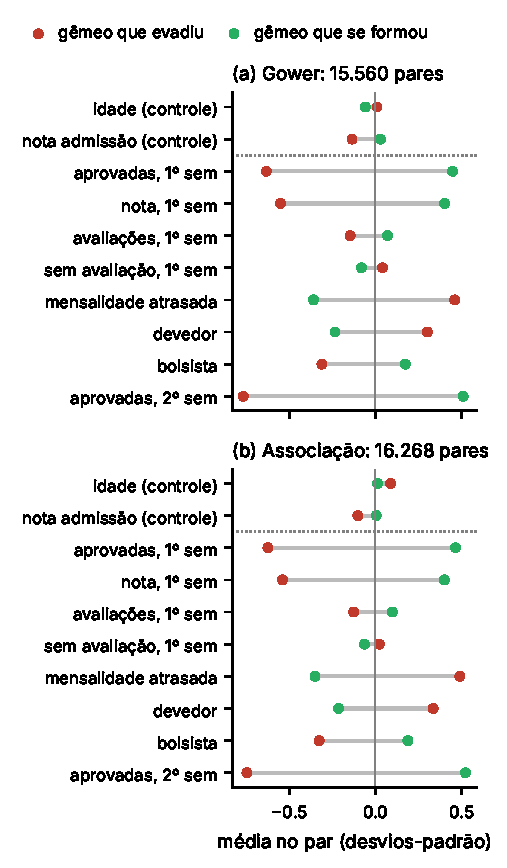
\includegraphics{figuras/11_gemeos_destinos_diferentes.pdf}
\caption{Pares de vizinhos no grafo da matrícula com desfechos opostos, pela distância (a) de Gower e (b) por associação: média padronizada do aluno que evadiu (vermelho) e do que se formou (verde). As duas primeiras linhas são controles.}
\label{fig-gemeos}
\end{figure}

\subsection{Discussão e dificuldades}

\textbf{H1 se confirma}: o grafo é homofílico e as comunidades separam a evasão muito acima do acaso nas três janelas, nas duas distâncias ($p = 0{,}001$ em todos os testes de permutação). \textbf{H2 se confirma em parte}: a associação gera comunidades mais coesas ($Q$ maior) em todas as janelas, mas melhora a separação dos desfechos com clareza só no 1º semestre (V de 0,58 contra 0,46; AUC 0,06 maior em todas as divisões); nas outras janelas o ganho é marginal, e a GraphSAGE não muda com a distância. \textbf{H3 se confirma}: a GraphSAGE supera o Leiden em 98\% a 100\% das divisões, nas três janelas. Os dois métodos se complementam: a GraphSAGE ordena o risco de cada aluno, e o Leiden organiza os alunos em grupos concretos e interpretáveis, como o de pais com escolaridade desconhecida. O custo é viável: a matriz de distâncias ocupa 50 MB ($O(n^2)$) e leva de 3 a 22 s; o kNN, cerca de 1 s; o Leiden, menos de 1 s; e cada treino da GraphSAGE, de 5 a 9 s (CPU, 1 \textit{thread}). A avaliação comum completa (50 divisões) leva cerca de 15 minutos por janela. As dificuldades foram reimplementar e validar a distância por associação em Python, tornar o Leiden reprodutível (kNN determinístico e semente fixa) e o custo de repetir a avaliação 50 vezes em três janelas.
